\section{Plant Distribution Analysis and Reproduction}

As mentioned previously, running a simulation using the ecosystem simulator to generate valid plant distributions can be a lengthy process (see section \ref{subsec:ecosytem_performance}). This processing time depends on the plant count and the resolution of the simulation window. The simulation illustrated in figure \ref{fig:ecosimulator_test_plant_count}, for example, took four and a half minutes to run.\\

The area to be covered by vegetation on the terrain, and therefore for which valid plant distributions created, is much larger than the hundred by hundred metre simulation window used in the ecosystem simulator. There are three obvious ways the ecosystem simulator could be used to generate vegetation for larger areas: \textit{Setting the simulation window to the area which must be covered}, \textit{decreasing the resolution of the simulation window} and by \textit{repeating the output of the hundred by hundred metre distribution (tiling)}. Each come with major setbacks, however, as \textit{increasing the simulation} window will further increase the processing time, \textit{decreasing the resolution} would impact the resulting realism and \textit{tiling} would create repetitive vegetation.\\

To attempt to generate vegetation which is coherent with that produced with the ecosystem but on a larger scale whilst minimizing impacts on performance and realism, the plant distribution output by the ecosystem simulator is analysed for later reproduction. The analysis and reproduction process are discussed in \textit{Analysis} and \textit{Reproduction} respectively.\\

The analysed distribution data, as well as permitting larger scale reproduction, can also be used as a cache mechanism to bypass future runs of the same ecosystem simulator run. Details on how this is implemented are discussed in \textit{Caching Distribution Data}.

To conclude this section, input exemplars will be analysed and the resulting reproduction(s) evaluated.

\subsection{Distribution Analysis}

\textit{Radial distribution analysis}, as described in section \ref{subsubsec:radial_distribution_analysis}, is performed on the output of the ecosystem simulator to grasp its core characteristics. Each plant instance acts as a single point and the different species represent the individual categories when performing the analysis. Customizations to the generic analysis algorithm are performed, however, to better suit the purpose of analysing plant distributions. Each are discussed separately below in: \textit{Generating the category hierarchy}, \textit{Category Dependency Analysis} and \textit{Point-size Analysis}. In \textit{Configuration Parameters} are discussed the parameters used. To conclude, the performance of the distribution will be discussed in \textit{Performance}.

\subsubsection{Generating the category hierarchy} \label{subsubsec:generating_cat_hierarchy}

During the reproduction phase, distributions for each category are created sequentially. One a valid distribution is created for a given category, it is static and \textbf{does not} change whilst points of other categories are being plotted. For this reason, the category hierarchy plays a vital role and has a big impact on the final distribution. A side effect of this hierarchical approach is that pair-correlation histograms do not need to be generated for each category pair combinations but only for combinations for which the target category is under or equal to the source category in the hierarchy.\\

Because taller plants will potentially have a canopy which shades and influences the position of smaller plants, it is important these be generated first during reproduction. For this reason, the hierarchy is generated according to the average height of the represented plant specie in descending order.

\subsubsection{Category Dependency Analysis} \label{subsubsec:category_dependency_analysis}

Shade-loving plants will appear under the the shaded canopies of taller plants (see section \ref{subsubsec:shade_loving_test}). When analysing the distance of these shade-loving plants to the plant's which shade them during the analysis phase, a new \textit{negative-bin} is created.\\

During reproduction, the taller plants will be generated first because they are classed higher in the hierarchy (see section \ref{subsubsec:generating_cat_hierarchy}). However, this does not guarantee all shade-loving plants will be placed in the shaded canopy of other plants as if a shade-loving plant is placed at a distance larger than \textit{R$_{max}$} to any other plant instance, it is attributed a strength of one and is therefore deemed valid. It is essential to attribute a strength of one in such condition to permit plant propagation. A solution to this problem would be to make \textit{R$_{max}$} large enough to cover the entire simulation window. This is extremely wasteful in terms of computational resources however and, as such, another solution is used here; When the pairwise histograms have been generated for a given category \textit{A}, they are analysed sequentially to check whether or not all instances appear within the \textit{negative-bin} of the other category (specie). The specie \textit{A} is deemed \textbf{dependent} on all categories for which this is true and, during reproduction, will have to be placed within the radius of one of them to be deemed valid.

\subsubsection{Point-size Analysis}

As well as the position of individual plants, an important property of the ecosystem simulator output is plant size. In order to reproduce appropriately sized plants, this must also be analysed. To do so, the \textit{minimum} and \textit{maximum} canopy radius and height for each category are also analysed.

\subsubsection{Configuration Parameters}

The \textit{radial distribution analysis} requires the following configuration parameters: \textit{R$_{min}$}, \textit{R$_{min}$} and \textit{bin-size}. Details on each parameter can be found in section \ref{subsubsec:radial_distribution_analysis}.\\

Increasing the analysis range [\textit{R$_{min}$}, \textit{R$_{max}$}] and decreasing the \textit{bin-size} will impact performance but potentially increase the accuracy of the analysis and finding optimal values for these parameters depends on the properties of the points being analysed.\\
It is unnecessary to have too large of an analysis range as the impact a plant has on it's surrounding is finite. This impact radius varies however and is dependent on specie size. In order to cater for different species of different sizes and therefore with different impact radii, R$_{max}$ is dynamic and limited to \textbf{two metres} passed the extremity of the plant's canopy.\\
The bin-size doesn't influence performance as severely as the analysis range, however, as it has no impact on the number of points that need to be processed. Smaller bin sizes will result in less points being processed per bin and, therefore, a less accurate representation of the distribution variation with distance. Because smaller bins will result in a smaller number of points, also, the analysis will be more sensitive to noise. A bin size of \textbf{twenty centimetres} is used as it strikes a good balance between accuracy and point count per bin. \\

\subsubsection{Performance} \label{subsubsec:analysis_performance}

In order to generate the necessary analysis data, each point (plant) must be iterated over and the distance measured from it to all other points within a radius of \textit{R$_{max}$}. As a consequence, the analysis time is directly correlated to plant density and, therefore, plant count within the hundred metre analysis window. To determine the correlation between plant density and analysis time, test distributions are generated of various densities using the ecosystem simulator which are subsequently analysed and the time to do so, measured. Because the number of histograms that need to be generated depends on the number of categories to be analysed, one would easily assume that the processing time is also correlated to the category count. This is \textbf{not} the case however and only point density influences analysis performance. To demonstrate this, the various plant densities are generated containing one, two and three distinct categories.The results plotted in figure \ref{fig:analysis_perf} indicate an exponential correlation between plant count and processing time and a quicker analysis time when points are split into multiple categories. Although the correlation is exponential, the most extreme scenario (over ninety thousand points of a single category) is processed in a manageable time of just under two seconds. 

\begin{figure}
\center
	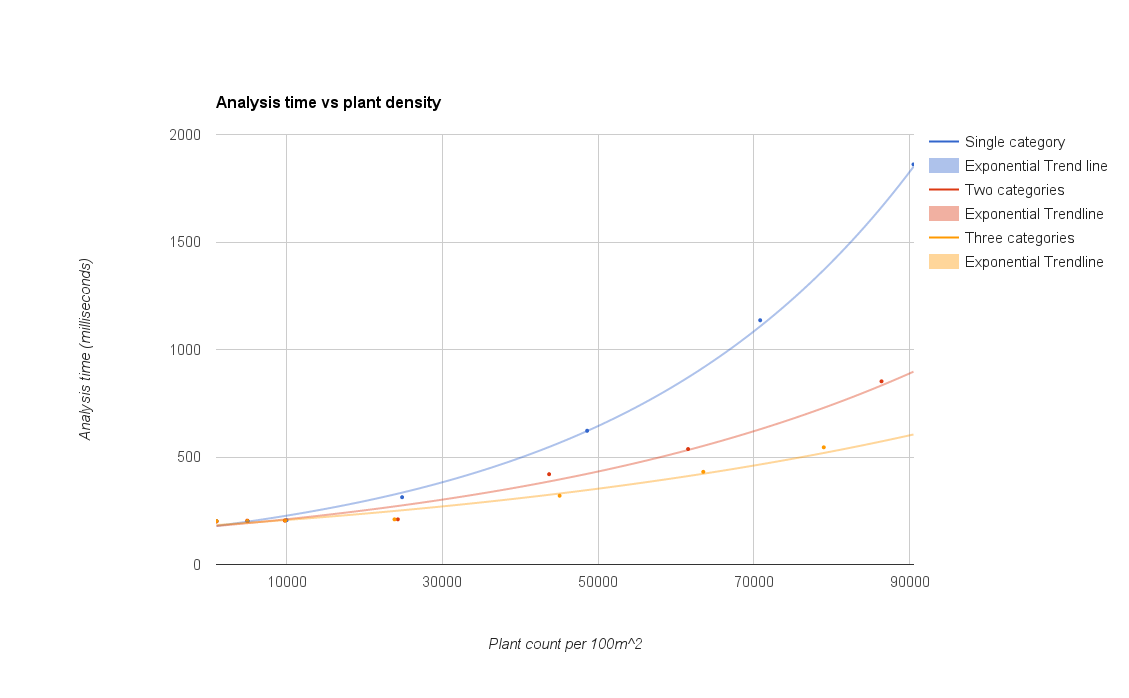
\includegraphics[width=\textwidth]{radial_distribution_analysis_performance.png}
	\caption{ Distribution analysis time based on aggregate plant density for single category (blue), two categories (red) and three categories (yellow).}	
	\label{fig:analysis_perf}
\end{figure}

\subsection{Reproduction}

The purpose of the analysed radial distribution data is to later use it to reproduce similar distributions on larger scales. To do so, the same reproduction technique described in section \ref{subsubsec:radial_distribution_analysis} is employed with slight nuances described below, namely: \textit{Matched-density initialization} and \textit{Iterative point moving}.\\

The radial distribution data generated to test the analysis performance above (section \ref{subsubsec:analysis_performance}) is used to test the reproduction performance.

\subsubsection{Matched Density Initialization}

Rather than employ a birth-and-death technique like that described in section \ref{subsubsec:radial_distribution_analysis}, where a point is added, the aggregate strength of the distribution calculated and the new point accepted with a calculated probability, matched-density initialization is employed. This involved generating a fixed number of points for each category so that their density matches that of the analysed density. The only requirement is for the aggregate strength of the distribution to be non-zero. In other words, the distribution does not need to be strongly matched, but valid.

\subsubsection{Iterative Point Moving} \label{subsubsec:iterative_point_moving}

When points of a given category have been initialized and the required density reached, iterative point-moving is performed where each added point is iterated over and moved to two random locations. The new distribution strength is calculated after each move and the best scoring move is accepted with probability \textit{P$_{acceptance}$}, calculated using equation \ref{eq:reproduction_probability_acceptance}. 

\begin{equation}
\centering
P_{acceptance} = \frac{Strength_{n+1}}{Strength_{n}}
\label{eq:reproduction_probability_acceptance}
\end{equation}
Where:
\begin{itemize}
\item \textit{Strength$_{n+1}$} is the aggregated distribution strength after the move.
\item \textit{Strength$_{n}$} is the aggregated distribution strength before the move.
\end{itemize}

\subsubsection{Performance}

The reproduction area and point density are two properties which greatly affect performance. Although both effect the number of points to reproduce and, therefore, the reproduction time, because an increase in density will lead to more points within R$_{max}$ of any given source point, given a fixed plant count, performance should increase with area. To determine to what extent and the correlation between plant density, reproduction area and performance, test reproductions are performed using the analysis data generated when performance testing the analysis stage (section \label{subsubsec:analysis_performance}).

As seen in figure \ref{fig:reproduction_density_area_perf} which plots the reproduction performance based on point density for various reproduction areas, the correlation between plant density and reproduction time is exponential. It also shows the increase to be more accentuated when reproducing larger areas. This is expected, however, as larger areas will require more points to be added in order to meet the required density.\\

\begin{figure}
\center
	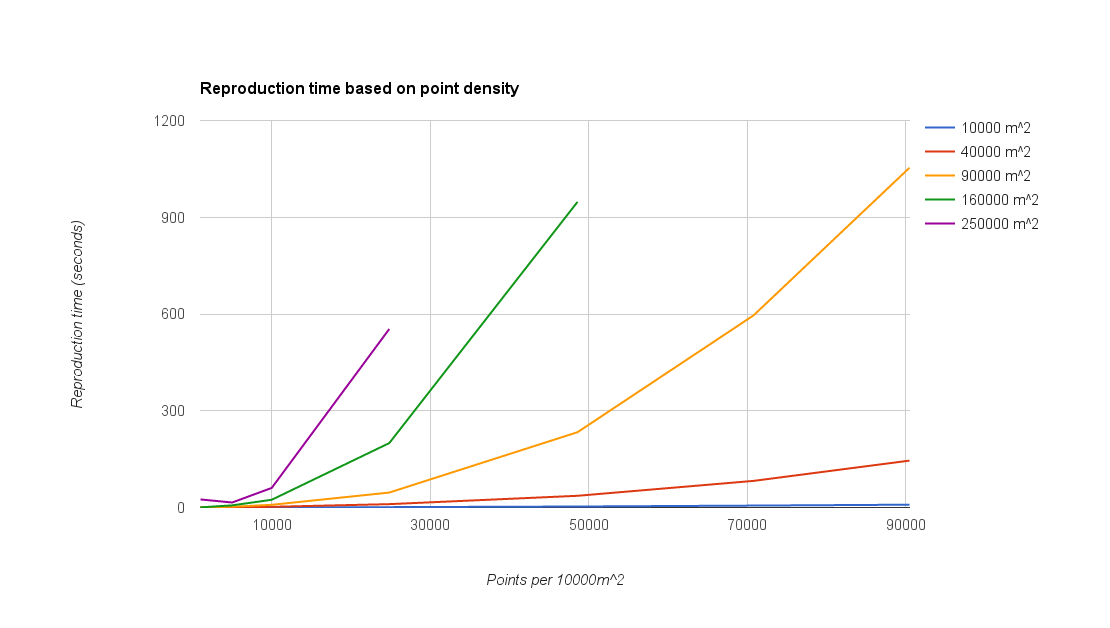
\includegraphics[width=\textwidth]{radial_distribution_reproduction_area_and_density_perf.png}
	\caption{ Reproduction time based on point density for different reproduction areas.}	
	\label{fig:reproduction_density_area_perf}
\end{figure}

Using the test data generated for figure \ref{fig:reproduction_density_area_perf}, it is possible to plot the reproduction time based solely on plant count for various densities (see figure \ref{fig:reproduction_plant_count_perf}). It shows the correlation between plant count and reproduction time to be linear and dependent on point density. The reason it is sensitive to plant density is because the denser the points are the the more of them will be within a distance of R$_{max}$ and therefore need ot be taken into consideration when calculating the strength of the distribution. In order to keep reproduction times manageable, the reproduced plant count is limited to half a million. If large areas need to be reproduced with a plant count higher than this limit, repeating/tiling is performed. Table \ref{tab:maximum_reproduction_areas} shows the maximum reproduction areas that can be achieved for different plant densities. Although the repetition (tiling) performed will increase for denser distributions, it will not necessarily be more noticeable as denser distributions will tend to have less distinct patterns and be more closely correlated to random.\\

\begin{figure}
\center
	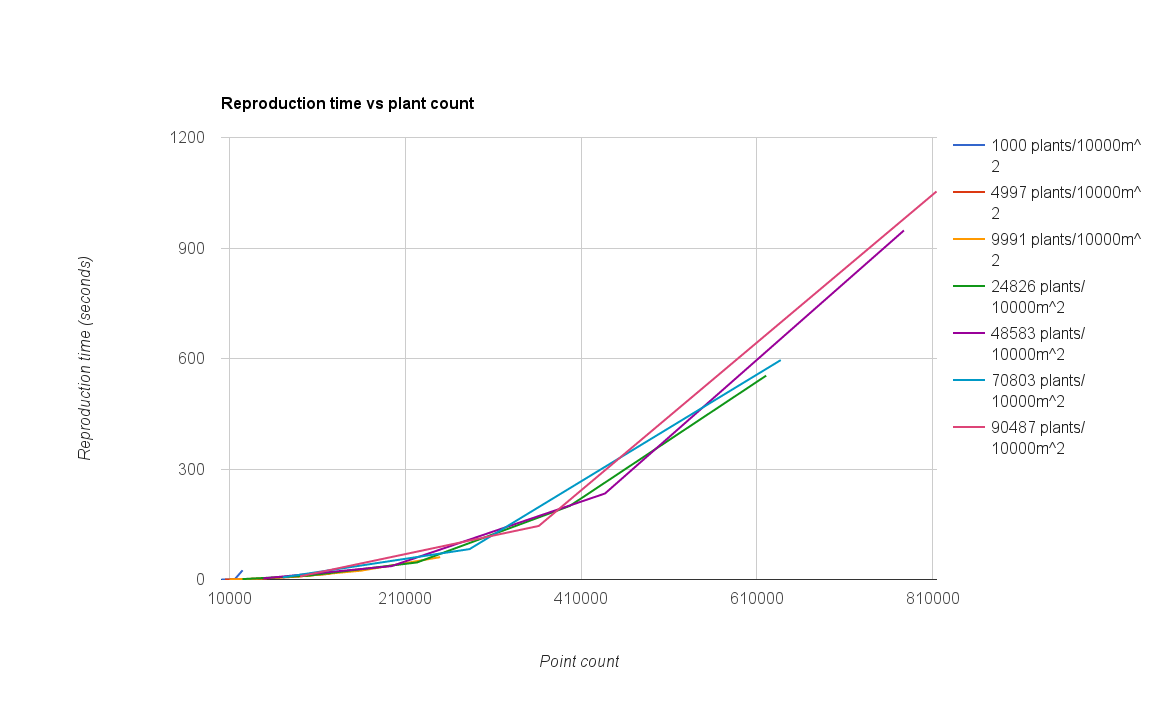
\includegraphics[width=\textwidth]{radial_distribution_reproduction_plant_count_perf.png}
	\caption{ Reproduction time based on point count for different densities.}	
	\label{fig:reproduction_plant_count_perf}
\end{figure}

\begin{table}[]
  \centering
	    \begin{tabular}{|p{7cm}|p{8cm}|}
		\hline
		\textbf{Points per 10000m$^{2}$} & \textbf{Maximum reproduction area (m$^{2}$)}\\
		\hline
		5000	  &  1000000\\
		\hline
		10000	  &  500000\\
		\hline
		15000 &	333333\\
		\hline
		20000 &	250000\\
		\hline
		25000 &	200000\\
		\hline
		30000 &	166666\\
		\hline
		35000 &	142857\\
		\hline
		40000 &	125000\\
		\hline
		45000 &	111111\\
		\hline
		50000 &	100000\\
		\hline
		55000 &	90909\\
		\hline
		60000 &	83333\\
		\hline
		65000 &	76923\\
		\hline
		70000 &	71428\\
		\hline
		75000 &	66666\\
		\hline
		80000 &	62500\\
		\hline
		85000 &	58823\\
		\hline
		90000 &	55555\\
		\hline
		95000 &	52631\\
		\hline
		100000 & 50000\\
		\hline
		\end{tabular}
		\caption{Maximum reproduction area for given plant densities}
	  \label{tab:maximum_reproduction_areas}
\end{table}

\subsection{Caching Distribution Data}

In order to prevent repeated costly runs of the ecosystem simulator for identical resource parameters, the analysed distribution data is stored and tracked in a database. This way, if a plant distribution is requested for a simulation which has already been run, the ecosystem simulator is bypassed entirely and the stored distribution data used. A custom binary file format is used in order to save space when storing the necessary analysed distribution data.

\subsection{Results}

The important properties of the input exemplars which must be reproduced are: \textit{inter and intra specie separation}, \textit{plant size} and \textit{specie densities}. To ensure these are accurately reproduced, an ecosystem simulator run is performed containing \textit{shade-loving}, \textit{shade intolerant} and \textit{canopy plants}. The resulting plant distribution is subsequently used as input exemplar to stress test the distribution analyser and reproducer. Figure \ref{fig:radial_dist_test} shows an overview and zoomed subsection of the input exemplar along with it's associated reproduction. From this, along with the point count of individual species, it is possible to conclude that point density and point size is accurately replicated. To determine whether intra and inter-specie spacing is accurately reproduced, the reproduction distribution is re-analysed in order to produce the pair correlation histograms of the reproduced distribution. The original and reproduced histograms are then compared to ensure they follow similar trends (see figure \ref{fig:hisogram_comp}). Important properties to note which are accurately reproduced are:
\begin{itemize}
\item No plants appear within the radius of the shade-loving (category 6) and shade-intolerant plants (category 5)
\item The density of shade-intolerant plants (category 5) drastically decreases within the radius of canopy plants (category 9).
\item The density of shade-loving plants (category 6) drastically decreases within the radius of canopy plants (category 9). Note that in both the original and reproduction, all shade-loving plants appear within the radius of a canopy plants as the categories are dependent (see section \ref{subsubsec:category_dependency_analysis}). The variation in histogram values between the two is caused by the positioning of other nearby canopy plants.
\item The density decreases drastically for canopy plants within the canopy of other canopy plants (category 9) as it blocks access to available illumination.
\end{itemize}

Note that the pair correlation histogram of the shade-loving specie with itself (category 6 and 6) is substantially different between original and reproduction. The reason for this is because during the ecosystem simulator, seeding is performed from existing plant instances which will lead to the clustering of plants under the same canopy. During iterative point-moving (see section \ref{subsubsec:iterative_point_moving}, the probability of shade-loving plants to cluster under neighbouring canopy plants is very slim, however, and dispersion under all present canopy plants is much more likely.

\begin{figure}
\center
	\includegraphics[width=\textwidth]{radial_distribution_test_general_comp.png}
	\caption{ Distribution analysis and reproduction test: Input exemplar overview (top-left), reproduction overview (top right), zoomed input exemplar (x 10), zoomed reproduction (x 10). }	
	\label{fig:radial_dist_test}
\end{figure}

\begin{figure}
\center
	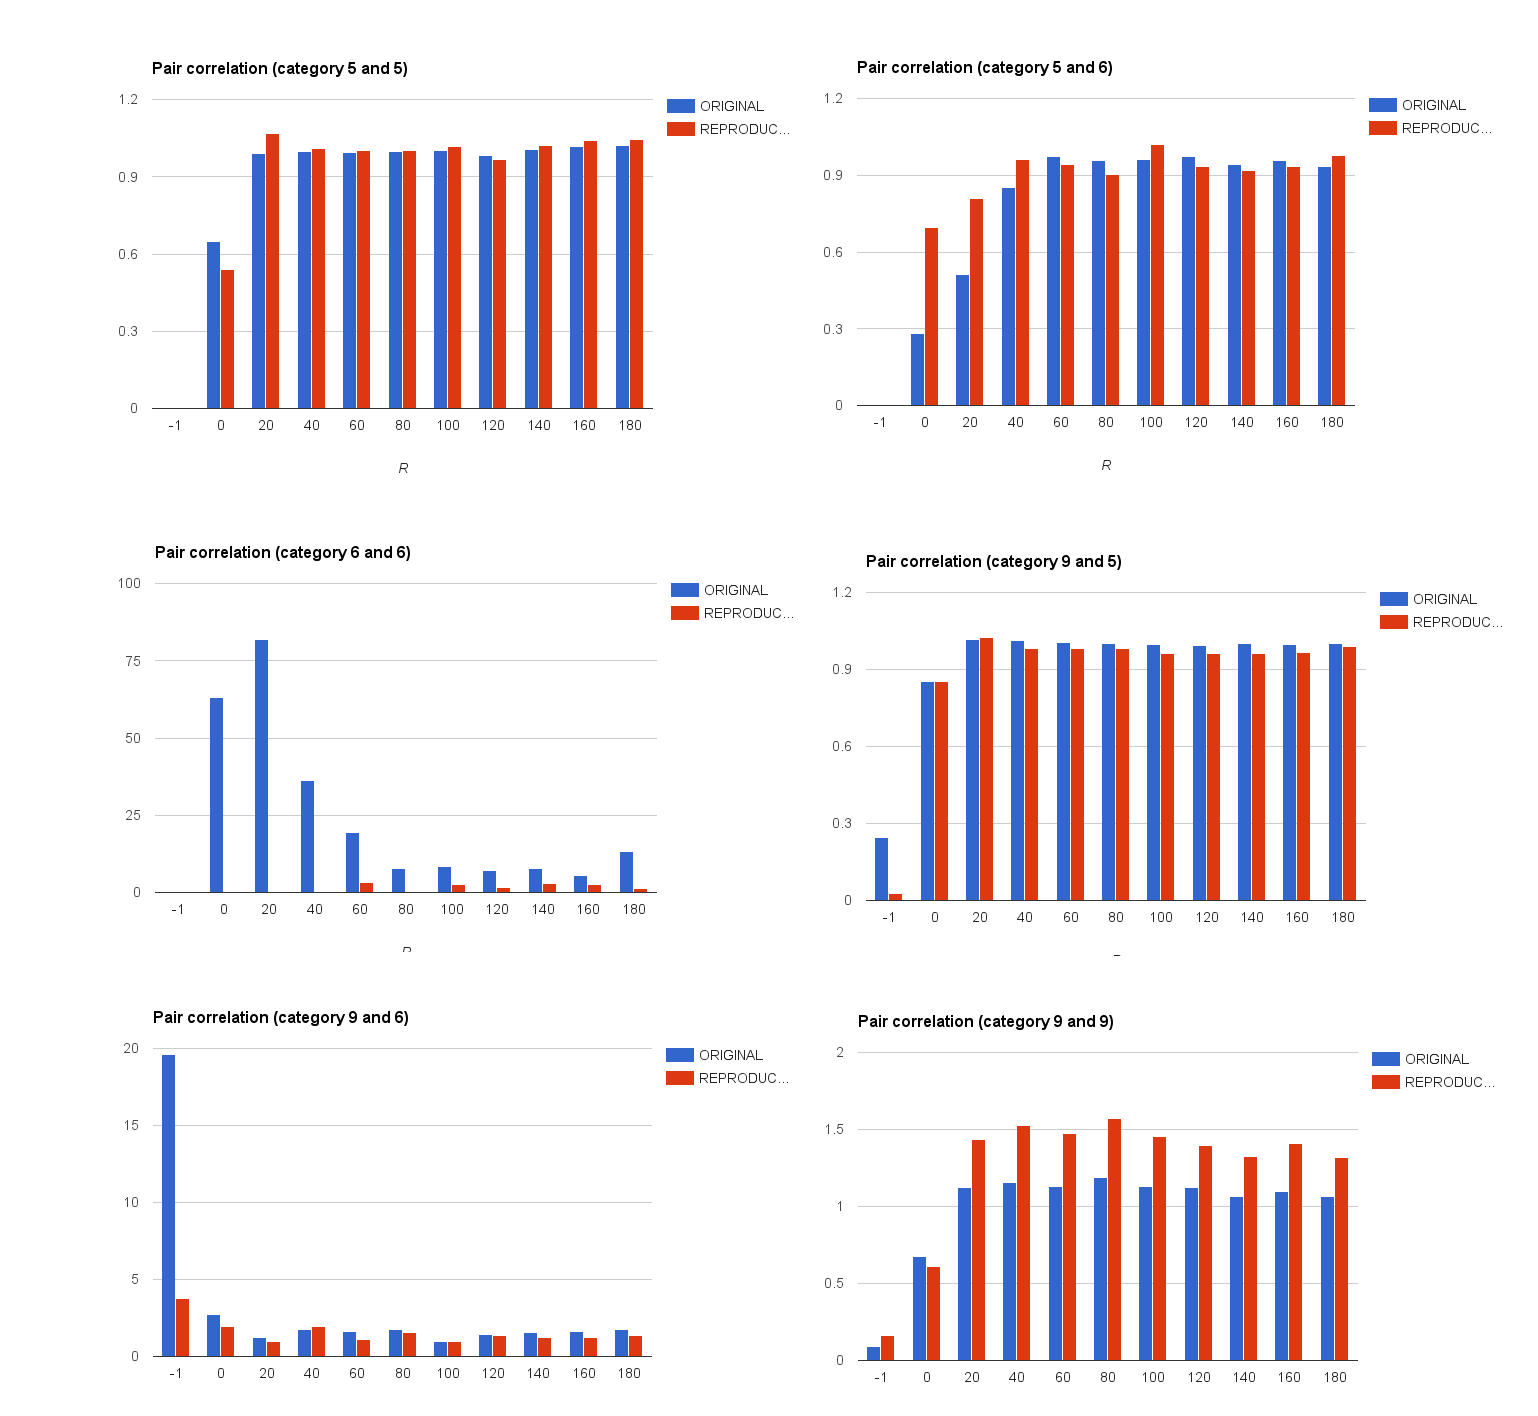
\includegraphics[width=\textwidth]{radial_dis_reprod_test_hist_aggregated.png}
	\caption{ Original (blue) and reproduced (red) pair correlation histograms for different bins where category 6 is a shade-loving, category 5 is shade intolerant and category 9 is a canopy specie. Bin sizes of -1 signify the target category is within the radius of the source.}	
	\label{fig:hisogram_comp}
\end{figure}
